\subsection{Raman beams design}
We generate Raman coupling with $\lambda \approx {\rm 790nm}$ laser. The recoil vector of the laser is 
\begin{equation}
   k_{\rm r} = \frac{2\pi}{\lambda}.
\end{equation}
When two Raman beams intersect at an angle $\theta_R$ as shown in Fig.~(\ref{fig:raman_design}), the two photon recoil vector is
\begin{equation}
    \kr = k_{\rm r}\sin{\frac{\theta_R}{2}}.
\end{equation}
As shown in Fig.~(\ref{fig:Dispersion relations}c), the detuning between states $\ket{q+\kr,\uparrow}$ and $\ket{q-\kr,\downarrow}$ is
\begin{equation}
    \Delta(q) = \frac{2\hbar^2q\kr}{m} + \delta.
\end{equation}
$\delta$ here is the detuning between two Raman beams and $\Delta(q)$ increases with $\kr$. As described in Sec.~(\ref{soc}), one step in the process we prepare the SOC quasimomentum state $\ket{q_0,-}$ is adiabatic evolution. We achieve this by ramping up the Raman coupling strength from zero to $\Or$ on a time scale slow compared to $\hbar/\Delta(q_0,0)$. In experiment, we prefer to ramp up Raman coupling fast, limited by the lifetime of BEC, but still slow compare to $\hbar/\Delta(q_0,0)$. For this reason, we want to make $\kr$ as large as possible. In this design, it means large enough intersection angle $\theta_R$. On the other hand, we also want $\kr$ to be small enough that $k_c/\kr$ is large enough the speckle potential can couple more energy matching stats shown as the circles in Fig.~(\ref{fig:Dispersion relations}). Here $k_c$ is the cut off in the PSD of the speckle potential. In our experiment, the two Raman beams and the speckle beam are focused to the atoms by the same lens $L_1$, at the largest $\theta_R$, $k_c/\kr \approx 3$. 

For the above two reasons, there is a trade off between small and large $\theta_R$, we need to find out the best angle by experimentally test. So for the optical design, we need to be flexible in changing the angle. As shown in Fig.~(\ref{fig:raman_design}), we use a triangular prism to combine the two Raman beams and align them to be parallel. The triangular prism is put on a transnational stage which can move in the perpendicular direction of the two incident Raman beams. By moving the prism, the distance between the two Raman beams can be changed and the distance is map to the distance at lens $L_1$ which determines the angle $\theta_R$.

\begin{figure*}
    \centering
    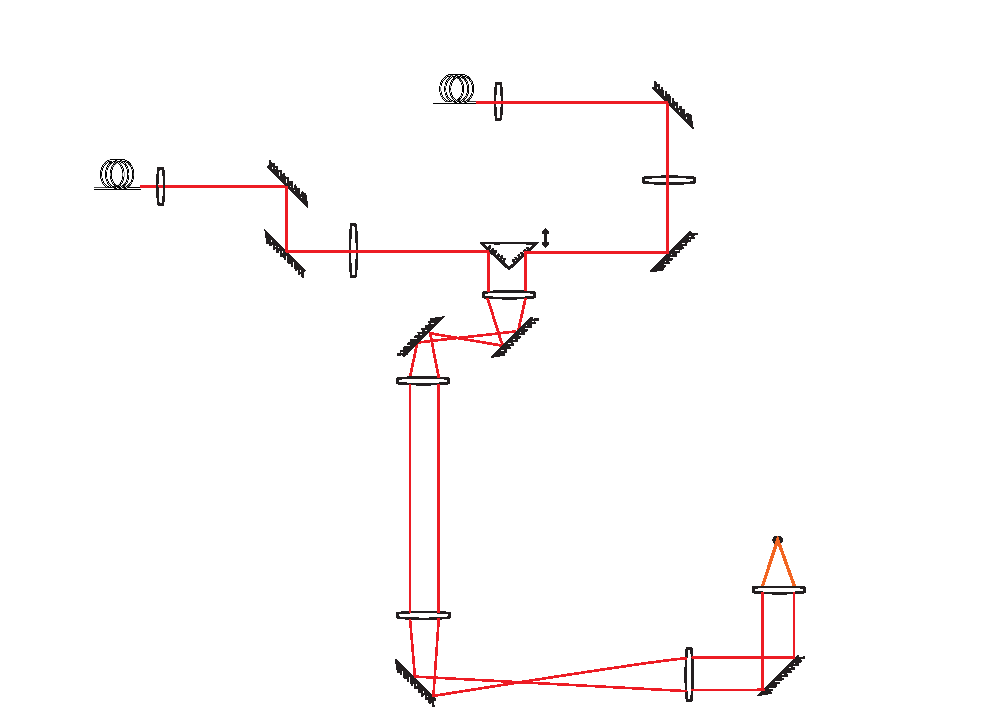
\includegraphics{Chapter6_secs/Raman_design.pdf}
    \caption{Raman beams design. The optical diagram of Raman beams. We use a triangular prism to align two Raman beams, the distance between two Raman beams at the prism is mapped to the distance at the lens $L_1$ by two relay imaging systems. The prism is put on a transnational stage which can move in the perpendicular direction of the two incident Raman beams. By moving the prism, the distance between the two Raman beams can be changed which determines the angle $\theta_R$.}
    \label{fig:raman_design}
\end{figure*}